According to the World Health Organization (WHO) \cite{oms2018},
cardiovascular diseases have remained the leading
deaths causes globally in the last 15 years. 
It is estimated that 15.2 million people died from CVD in 2016,
representing 26.7\% of all deaths in the world. 
In Brazil, about 38\% of deaths due to CVD is in the procutive age range
(18 to 65 years) and the estimated
costs of CVD were R\$ 37.1 billion
in 2015, that is, 0.7\% GDP \cite{siqueira2017}.

\medskip
About 60\% of CVD deaths
occurred due to coronary artery disease (CAD).
The main cause of CAD is the atherosclerosis which consists of
the accumulation of fatty plaques inside the artery wall causing
a decrease in lumen diameter.
The Atherosclerosis can be prevented with a change in harmful habits
such as: cigarette smoking, physical inactivity/low fitness and poor dietary habits \cite{spring2013}.
For a corrective approach, however, two treatments can be performed:
the \textit{Coronary Artery Bypass Sugery} (CABG) or a 
procedure minimally invasive where a wire tube is placed.
The procedure development 
originates in 1964 with Dotter and Judkins \cite{dotter1964}, where they
introduced a new technique for obstructed femoral artery treatment
 due to atherosclerosis. This technique is
known as \textit{percutaneous transluminal angioplasty}.
Such procedure is presented applicable to
 other arteries, including the coronary artery.


\medskip
In 1979, Gruntzig, Senning and Seigenthaler \cite{gruntzig1979}
 performed the percutaneous transluminal technique in the artery
coronary artery using a balloon catheter in order to dilate the site
with stenosis. 
The procedure was performed on 50 patients for 18 months and
satisfactory results were presented, mainly with patients with only
a single artery with sterosis. 
Such procedure is known as \textit{Coronary Angioplasty
Percutaneous Transluminal} (PTCA).

\medskip
Although PTCA using a balloon has shown satisfactory results,
over time, the artery presented restenosis. 
In 1987, Sigwart et al. \cite{sigwart1987}
present the result of implanting a prosthesis made of a 
self-expanding stainless steel mesh in the femoral and 
coronary arteries of 25 patients who cases of restenosis. 
The prosthesis proved to be a
interesting way to solve restenosis. 
This prosthesis was called \textit{stent}.


\medskip
In 1994, Serruys et al. \cite{serruys1994} present a comparison between PTCA procedures
using an balloon and stent implantation. 520 patients were analyzed,
where 262 patients with implanted stents and 258 patients with the
inflatable balloon. The clinical and angiographic results were better for the patients who had stent implantation to those who underwent the procedure only
using the balloon. Thus, the PTCA procedure with stent implantation
was confirmed as a more effective solution than PTCA using only the balloon.
However, a problem persisted: the restenosis. 
During the 1990s, researchers
sought to solve this problem. The \ref{procedimentos PTCA} presents the comparison between
PTCA procedures using the balloon and stent.

\begin{figure}[H]
     \begin{minipage}{.50\linewidth}
      \centering
      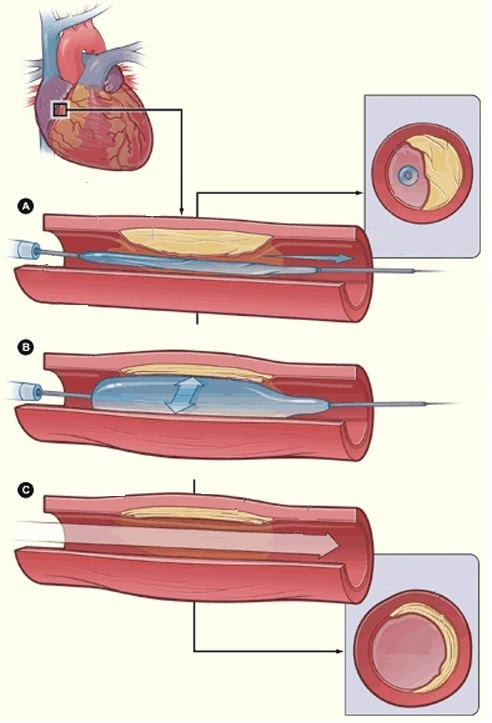
\includegraphics[scale=0.5]{./02_chaps/cap_review/figure/balloon.jpg}\\
      (a)
     \end{minipage}%
     \begin{minipage}{.50\linewidth}
      \centering
      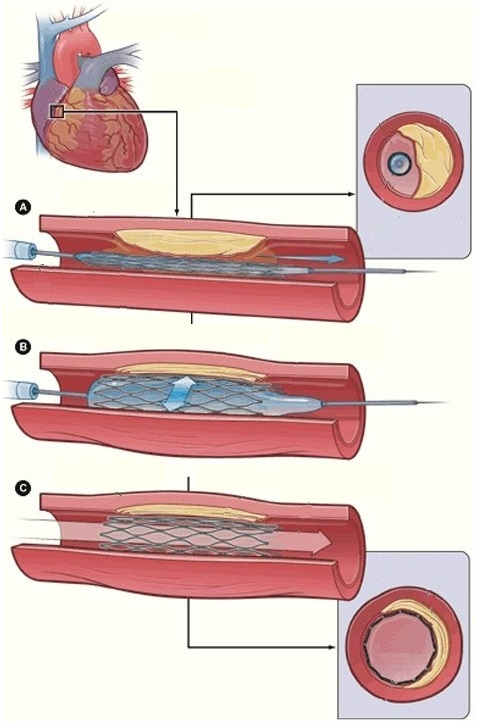
\includegraphics[scale=0.5]{./02_chaps/cap_review/figure/stent_bare.jpg}\\
      (b)
     \end{minipage}
     \medskip
     \caption{Comparison PTCA procedure:
              (a) balloon and
              (b) stent.}
     \label{procedimentos PTCA}
\end{figure}

\medskip
In 2001, Hwang, Wu and Edelman \cite{hwang2001} presented a simulation of stent implantation
coated with a drug in a coronary artery. 
The simulation presented the
close relationship between drug distribution and \textit{Peclet number}
in addition to the importance of developing geometries for stents that enhance
the diffusion of the chemical substance. 
Such procedure proved to be a promising option
for the treatment of atherosclerosis and reestonosis. 
This new type of stent
would be known as \textit{drug-eluting stent}.


\medskip
In 2009, Zunino et al. \cite{zunino2009} presented a complete overview
of mathematical models and finite element numerical simulation 
applied to the  modelling of drug eluting stens and 
of their interaction with
the coronary arteries, take into account the stent expansion,
fluid dynamics around the stent and drug release. The numerical
simulation shown recirculation zones downstream 
has important consequences on the drug release process.
The smooth and concave shape of stent contours shows that
part of the drug released and accumulated in the neighborbood
of the links is transported away and may affect the arterial
walls located downstream. However, for the case analyzed,
the authors concluded that the drug released into the lumem
does not significantly contribute to the permanent drug
deposition into the arterial wall and only an small fraction of
the total amount drug stored into the stent was effectively
delivered to the artery.


\medskip
In 2014, Bozsak, Chomaz and Barakat \cite{bozsak2014} propose a computational model of transport
of the drugs \textit{paclitaxel} and \textit{sirolimus} on the artery wall. Such drugs are
frequently used in drug-eluting stents. The model takes into account the structure in
multilayer of the artery wall and these layers were modeled as porous media.
Thus, the law of \textit{Darcy} was used to simulate the flow within the layers
of the artery. The simulation showed that the choice of the type of drug used
is a crucial parameter in the creation of the drug-eluting stent
due to transport in the artery wall.


\medskip
In 2016, Bukac et al. \cite{bukac2016} present a fluid-structure
interaction between a curved coronary artery with an implanted stent,
pulsatile blood flow and heart contractions. 
An finite element numerical simulation
was performed using ALE approach and the Navier-Stokes equations for
an incompressible, viscous fluid are used to model the blood flow.
The performance of the four commercially 
available stent geometries stent struts was evaluated based on the
pathobiologic parameters responses leading to restenosis 
in the curved coronary arteries and the horizontal sinusoidal of
\textit{Cypher stent struts} performed the best in terms of theses
parameters. However, on limitation of the model used in the work 
is that it does not account for the protrusion of stent struts into the
vessel lumen. Thus, the influence of small-scale vortices around
stent struts on wall shear stress was not studied.


\medskip
Recently, Wang et al. \cite{wang2017} present the simulation
 of blood flow in a coronary artery with atherosclerosis and
 drug-eluting stent placed. Blood is approximated as a Newtonian and
 monophase fluid and the governing equations were approximated
 according to the Finite Element Method. Several axisymmetric
 geometries were presented, including a real coronary artery.
 Such geometries were used for this current work, but modified
 for a two-dimensional approach. The simulations showed that
 the proposed simplified artery with atherosclerosis model
 produced similar results of velocity, pressure and concentration
 when compared to the real artery.

\medskip
The following year, Lucena et al. \cite{lucena2018} present 
the simulation of the transport of the drug \textit{sirolimus}
 on the wall of an artery modeled as a porous and anisotropic medium.
 Dissolution in the polymeric stent lining in addition to transport
 in the artery wall in an axysymmetric domain was considered.
 The government equations were approximated according to
 the Finite Element Method. The work showed that the evolution time
 of the transport process can be efficiently controlled by
 the mass diffusivity of the polymer. It is estimated that
 about 47\% of the drug is diffused in the lumen and is lost in
 the bloodstream. The spatial distribution of the drug, however,
 is greatly influenced by blood flow and the properties of 
the artery wall. Thus, such results are susceptible to the
 patient's health conditions.

\medskip
In 2019, Gudino, Oishi and Sequeira \cite{gudino2019} presented
the influence of non-Newtonian blood flow models on drug
diffusion from a coronary drug-eluting stent. 
The Oldroyd-B, Phan-Thien-Tanner and Giesekus viscoelastic models
were used to describe the fluid dynamics of blood and the finite
element method was used for numerical simulations. The simulations
shown the hemodynamics captured by each model are more significant
in the proximal recirculation zones. The comparison between the
newtonian and non-newtonian model were performed and
the results of total stress tensor as well as the drug concentration in the artery
wall showed significant differences between the models. 


\medskip
Over the past and current decade, several drug-eluting stents
 have been developed such as: \textit{Ravel} \cite{morice2002},
 \textit{Taxus I and Taxus II} \cite{grube2003} \cite{colombo2003},
 \textit{C-Sirius} \cite{schampaert2004},
 \textit{Smart} \cite{ardissino2004} and
 more recent ones as presented in \ref{stent drug}. 
Currently, a new generation of stents has been developed
 in which the entire structure is absorbed. 
Such a generation is known as \textit{bioabsorbable stent}, 
the use of this technology is not the subject of this work.


\begin{figure}[H]
  \centering
  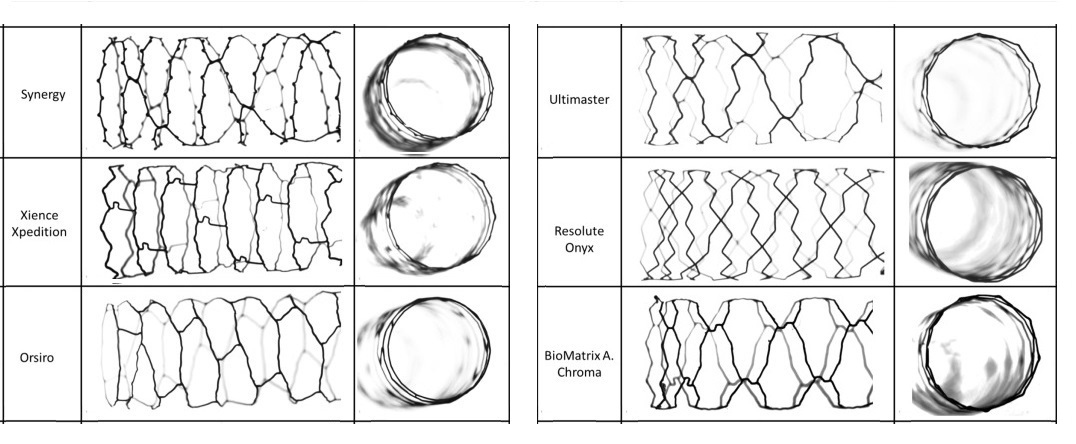
\includegraphics[scale=0.66]{./02_chaps/cap_review/figure/stent_drug.jpg}
 \caption{Several models of drug-eluting stent \cite{stent2016}.}
 \label{stent drug}
\end{figure}

